\documentclass[a4paper]{article}
% generated by Docutils <http://docutils.sourceforge.net/>
\usepackage{cmap} % fix search and cut-and-paste in Acrobat
\usepackage{ifthen}
\usepackage[T1]{fontenc}
\usepackage[utf8]{inputenc}
\usepackage{alltt}
\usepackage{amsmath}
\usepackage{color}
\usepackage{float} % float configuration
\floatplacement{figure}{H} % place figures here definitely
\usepackage{graphicx}
\setcounter{secnumdepth}{0}
\usepackage{longtable,ltcaption,array}
\setlength{\extrarowheight}{2pt}
\newlength{\DUtablewidth} % internal use in tables
\usepackage{textcomp} % text symbol macros

%%% Custom LaTeX preamble
% PDF Standard Fonts
\usepackage{mathptmx} % Times
\usepackage[scaled=.90]{helvet}
\usepackage{courier}

%%% User specified packages and stylesheets

%%% Fallback definitions for Docutils-specific commands

% class handling for environments (block-level elements)
% \begin{DUclass}{spam} tries \DUCLASSspam and
% \end{DUclass}{spam} tries \endDUCLASSspam
\ifx\DUclass\undefined % poor man's "provideenvironment"
 \newenvironment{DUclass}[1]%
  {\def\DocutilsClassFunctionName{DUCLASS#1}% arg cannot be used in end-part of environment.
     \csname \DocutilsClassFunctionName \endcsname}%
  {\csname end\DocutilsClassFunctionName \endcsname}%
\fi

% admonition (specially marked topic)
\providecommand{\DUadmonition}[2][class-arg]{%
  % try \DUadmonition#1{#2}:
  \ifcsname DUadmonition#1\endcsname%
    \csname DUadmonition#1\endcsname{#2}%
  \else
    \begin{center}
      \fbox{\parbox{0.9\linewidth}{#2}}
    \end{center}
  \fi
}
% basic code highlight:
\providecommand*\DUrolecomment[1]{\textcolor[rgb]{0.40,0.40,0.40}{#1}}
\providecommand*\DUroledeleted[1]{\textcolor[rgb]{0.40,0.40,0.40}{#1}}
\providecommand*\DUrolekeyword[1]{\textbf{#1}}
\providecommand*\DUrolestring[1]{\textit{#1}}

% inline markup (custom roles)
% \DUrole{#1}{#2} tries \DUrole#1{#2}
\providecommand*{\DUrole}[2]{%
  \ifcsname DUrole#1\endcsname%
    \csname DUrole#1\endcsname{#2}%
  \else
    % backwards compatibility: try \docutilsrole#1{#2}
    \ifcsname docutilsrole#1\endcsname%
      \csname docutilsrole#1\endcsname{#2}%
    \else%
      #2%
    \fi%
  \fi%
}

% title for topics, admonitions, unsupported section levels, and sidebar
\providecommand*{\DUtitle}[2][class-arg]{%
  % call \DUtitle#1{#2} if it exists:
  \ifcsname DUtitle#1\endcsname%
    \csname DUtitle#1\endcsname{#2}%
  \else
    \smallskip\noindent\textbf{#2}\smallskip%
  \fi
}

% hyperlinks:
\ifthenelse{\isundefined{\hypersetup}}{
  \usepackage[colorlinks=true,linkcolor=blue,urlcolor=blue]{hyperref}
  \usepackage{bookmark}
  \urlstyle{same} % normal text font (alternatives: tt, rm, sf)
}{}
\hypersetup{
  pdftitle={Línuleg algebra},
}

%%% Body
\begin{document}
\title{Línuleg algebra%
  \label{linuleg-algebra}}
\author{}
\date{}
\maketitle

Línuleg algebra er undirgrein stærðfræði sem fjallar um vigra og fylki, vigurrúm,
línulegar jöfnur og jöfnuhneppi, t.d. $5x + 3y = 13, x - y = 1$, línuleg
föll (eða línulegar varpanir), t.d. $f(x,y) = 2x + 3y$.
Meðal fleiri grunnhugtaka línulegrar algebru sem hér verða kynnt eru línulega
háð og óháð mengi vigra, grunnar, norm, horn milli vigra, auk þess sem fjallað verður um
ýmsa hagnýtingu línulegrar algebru. Oft tengist þessi hagnýting því að
vigrar og fylki eru notuð til að vinna með eða tákn gögn (\emph{data}) af ýmsu tagi.

Í nýlegri kennslubók um línulega algebru er fjallað um fjölbreytt
notkunarsvið svo sem leikjafræði, skógrækt, tölvugrafík, sneiðmyndatöku,
dulmálsfræði, erfðafræði, stofnstærðarspár, líkön af heyrn, netleit og andlitskennsl.

Þessi kafli byrjar á að rifja upp efni sem fjallað var um með \href{http://cs.hi.is/strei/linalg-1.pdf}{töflufyrirlestri} (sjá líka \emph{Námsefni-{}-Töflumyndir} í Canvas),
með stærðfræðilegri skilgreiningu á vigrum og fylkjum ásamt helstu aðgerðum sem
beita má á þessa hluti.


\section{Vigrar og fylki%
  \label{vigrar-og-fylki}%
}


\subsection{Skilgreining vigurs%
  \label{id1}%
  \label{skilgreining-vigurs}%
}

\emph{Vigur} (\emph{vector}) er runa af endanlega mörgum tölum sem notuð er sem ein heild
og oft gefið nafn sem er lítill bókstafur (t.d. $a$, $b$...). Vigur
með tölunum 1, 2 og 4 er ritaður:
%
\begin{equation*}
(1,2,4)\,\text{ e\eth a }\,[1,2,4]\,\text{ e\eth a }\,\begin{pmatrix}1\\2\\4\end{pmatrix}.
\end{equation*}
Fjöldi talna í vigri er kölluð \emph{vídd} (\emph{dimension}, eða \emph{size}) vigursins og
tölurnar í honum eru kallaðar \emph{stök} hans (\emph{elements}). Stakið í $i$-ta
sæti í vigri $a$ er táknað $a_i$. Vigur með $n$ stök er
stundum kallaður $n$-vigur, og mengi allra $n$-vigra er táknað
$\Bbb{R}^n$. Ef $a \in \Bbb{R}^n$ gildir sem sé
%
\begin{equation*}
a = (a_1, a_2, \ldots, a_n)
\end{equation*}
\DUadmonition[attention]{
\DUtitle[attention]{Attention!}

Þegar hugtakið \emph{vídd} er notað um tölvufræðilegt fylki (\emph{array}),
eins og rætt var í grein %
\raisebox{1em}{\hypertarget{id3}{}}\hyperlink{id2}{\textbf{\color{red}:numref:`um-orðið-fylki`}} merkir það fjölda vísa
(\emph{indices}) sem notaðir eru til að vísa í einstök stök (vigrar eru þannig
einvíð fylki), en þegar hugtakið er notað um vigur (hvort sem er í tölvufræði
eða stærðfræði) merkir það fjölda staka í honum. Í tölvufræði er reyndar
algengt að nota \emph{lengd} (\emph{length}) um fjölda staka í lista eða vigri, en af
því að það er líka notað um rúmfræðilega lengd vigurs höldum við okkur við
orðið vídd.

\DUadmonition[system-message]{
\DUtitle[system-message]{system-message}
\raisebox{1em}{\hypertarget{id2}{}}

{\color{red}ERROR/3} in \texttt{kafli04.rst}, line~48

\hyperlink{id3}{
Unknown interpreted text role \textquotedbl{}numref\textquotedbl{}.
}}
}

\DUadmonition[attention]{
\DUtitle[attention]{Attention!}

Í Numpy er fyrsta stak vigurs númerað 0, þannig að um vigur a með n
stök gildir   \texttt{a = np.array({[}a{[}0{]}, a{[}1{]}, ..., a{[}n-1{]}{]})}
}

Í fyrrnefndum \href{http://cs.hi.is/strei/linalg-1.pdf}{töflufyrirlestri} má finna
nokkur dæmi um notkun vigra, meðal annars til að tákna ýmis gögn.


\subsection{Skilgreining fylkis%
  \label{skilgreining-fylkis}%
}

\emph{Fylki} (\emph{matrix}) er tafla með tölum sem notuð er sem ein heild og oft
gefið nafn sem er stór bókstafur (t.d. $A$, $B$...). Taflan er
ýmist sett innan sviga eða hornklofa:
%
\begin{equation*}
A = \begin{pmatrix}1 & 2 & 3\\6 & 7 & 8\end{pmatrix} =
\begin{bmatrix}1 & 2 & 3\\6 & 7 & 8\end{bmatrix}
\end{equation*}
Fylki hafa tiltekinn fjölda af \emph{línum} (eða \emph{röðum}) og (\emph{dálkum}) (\emph{rows} og
\emph{columns}) og fylki með $m$ línum og $n$ dálkum er sagt hafa \emph{stærð}
(\emph{size}) $m \times n$: Fylkið $A$ að ofan er $2 \times 3$
fylki (lesið 2 sinnum 3 fylki, eða á ensku \emph{2 by 3} matrix). Einstakar tölur í
fylki eru kölluð \emph{stök} og staðsetning þeirra er \emph{sæti}, þannig að talan 8 í
fylkinu $A$ er sögð vera í sæti $(2,3)$ (línan kemur á undan
dálkinum). Stak í línu $i$ og dálki $j$ í fylki $A$ er táknað
$a_{ij}$; fyrir $A$-ið að ofan gildir $a_{23} = 8$.

% Sýnidæmi

\DUadmonition[important]{
\DUtitle[important]{Important}

\begin{enumerate}
\renewcommand{\labelenumi}{(\arabic{enumi})}
\item Birgðastöðu af vörum mætti tákna með fylki, t.d. gætum við látið
$b_{ij}$ tákna birgðir af vöru $i$ á degi $j$; þá væri
$B$ birgðafylki.

\item Blóðþrýsting $n$ einstaklinga mætti tákna með $n \times 2$
fylki $P$, þar sem fyrri dálkurinn gefur slagþrýsting
(\emph{systolic}) og sá seinni aðfallsþrýsing (\emph{diastolic}).
\end{enumerate}
}

% Æfing

\DUadmonition[hint]{
\DUtitle[hint]{Hint}

Blóðþrýsingur þriggja einstaklinga mældist 120/80, 140/90 og 105/65.

\begin{enumerate}
\renewcommand{\labelenumi}{\alph{enumi}.}
\item Hvert er blóðþrýstingsfylkið $P$?

\item Hver er stærð þess?

\item Hvað er $p_{22}$?

\item Í hvaða sæti er 80?
\end{enumerate}
}


\subsection{Einfaldar vigur- og fylkjaaðgerðir%
  \label{einfaldar-vigur-og-fylkjaagerir}%
}

Vigra er hægt að leggja saman og draga frá hver öðrum og einnig má margfalda
vigur með tölu. Þetta er gert með því að beita tilsvarandi aðgerðum á einstök
stök. Ef $x$ og $y$ eru vigrar og $c$ er tala þá gildir:
%
\begin{align*}
u &= x + y\text{ er vigur me\eth  }u_i = x_i + y_i\\
v &= x - y\text{ er vigur me\eth  }v_i = x_i - y_i\\
w &= cx\text{ er vigur me\eth  }w_i = cx_i\text{ í }i
\end{align*}
Á sama hátt má leggja saman og draga frá fylki og margfalda þau með tölu: Ef
$A$ og $B$ eru fylki og $c$ er tala þá gildir:
%
\begin{align*}
U &= A + B\text{ er fylki me\eth  }u_{ij} = a_{ij} + b_{ij}\\
V &= A - B\text{ er fylki me\eth  }v_{ij} = a_{ij} - b_{ij}\\
W &= cA\text{ er fylki me\eth  }w_{ij} = ca_{ij}
\end{align*}
Þetta er nánar útskýrt í fyrrnefndum \href{http://cs.hi.is/strei/linalg-1.pdf}{töflufyrirlestri} þar sem líka eru gefin þrjú dæmi um
samlagningu vigra, sér í lagi vigra sem tákna færslur í rúmi.


\subsection{Reglur um vigur- og fylkjaaðgerðir%
  \label{reglur-um-vigur-og-fylkjaagerir}%
}

Um samlagningu og frádrátt vigra og fylkja gilda víxlregla og tengiregla
einnig gildir dreifiregla um margföldun með tölu. Ef
$x$, $y$ og $z$ eru vigrar, $A$, $B$ og $C$
eru fylki og $\alpha$ er tala þá gildir:
%
\begin{align*}
x + y &= y + x\\
A + B &= B + A\\
x + (y + z) &= (x + y) + z\\
A + (B + C) &= (A + B) + C\\
\alpha(x + y) &= \alpha x + \alpha y\\
\alpha(A + B) &= \alpha A + \alpha B
\end{align*}
og í stað $+$ má setja $-$.


\subsection{Innfeldi%
  \label{id6}%
  \label{innfeldi}%
}

\emph{Innfeldi} eða \emph{skalarmargfeldi} (\emph{inner product}, \emph{dot product})
tveggja $n$-vigra $x$ og $y$ er skilgreint sem
%
\begin{equation*}
x \cdot y = x_1 y_1 + \ldots + x_n y_n = \sum_{i=1}^n x_i y_i
\end{equation*}
Ef $x = (3,2)$ og $y = (4,5)$ fæst sem sé $x \cdot y = 3 \cdot
4 + 2 \cdot 5 = 22$.

\begin{quote}
\textbf{Regla:} Ef $x$ og $y$ eru rúmvigrar þá gildir:
%
\begin{align*}
&x \cdot y = 0 \text{ þá og því a\eth eins a\eth  } x \text{ sé hornréttur á } y\\
&x \cdot y > 0 \text{ þá og því a\eth eins a\eth  horni\eth  á milli } x \text{ og } y
\text{ sé hvasst }
\end{align*}\end{quote}

% Sýnidæmi

\DUadmonition[important]{
\DUtitle[important]{Important}

\begin{enumerate}
\renewcommand{\labelenumi}{(\arabic{enumi})}
\item Lát
%
\begin{align*}
v_i &= \text{vægi námskei\eth s } i = \frac{\text{ECTS-einingar
námskei\eth s } i}{\text{heildareiningar}} \\
e_i &= \text{einkunn í námskei\eth i } i
\end{align*}
Þá er vegin meðaleinkunn allra námskeiða gefin með innfeldinu $v
\cdot e$

\item Lát
%
\begin{align*}
s_i &= \text{söluver\eth  á einingu af vöru } i\\
m_i &= \text{selt magn af vöru } i
\end{align*}\end{enumerate}
}

% Æfing

\DUadmonition[hint]{
\DUtitle[hint]{Hint}

Einkunnir Jóns haustið 2019 voru sem hér segir

\begin{longtable*}[c]{|l|l|l|}
\hline
Námskeið & Ein. & Einkunn \\
\hline
Hagnýt stærðfræðigreining & 8 & 6.5 \\
\hline
Tölvunarfræði 1 & 6 & 9.0 \\
\hline
Stærðfræðimynstur & 8 & 7.0 \\
\hline
Vefforritun & 8 & 8.0 \\
\hline
\end{longtable*}

\begin{enumerate}
\renewcommand{\labelenumi}{\alph{enumi}.}
\item Ákvarðið vægisvigur $v$ og einkunnarvigur $e$

\item Notið innfeldi til að finna meðaleinkunn Jóns
\end{enumerate}
}

Um innfeldi gildir víxlregla, tengiregla fyrir margfeldi með
tölu og dreifiregla:
%
\begin{align*}
x\cdot y &= y\cdot x \\
a(x\cdot y) &= ax\cdot y \\
x\cdot(y + z) &= x\cdot y + x\cdot z
\end{align*}
hér eru $x$, $y$ og $z$ vigrar og $a$ er tala.


\subsection{Hornalína fylkis og bylting%
  \label{hornalina-fylkis-og-bylting}%
  \label{bylting}%
}

\emph{Hornalína} (\emph{diagonal}) fylkis liggur frá horninu efst t.v. og niður á ská til
hægri. Þannig inniheldur hornalína fylkisins
%
\begin{equation*}
\begin{pmatrix}1 & 2 & 3\\4 & 5 & 6\\7 & 8 & 9\end{pmatrix}
\end{equation*}
stökin 1, 5 og 9. Svokölluð bylting (\emph{transpose}) fylkis fæst með því að spegla
því um hornalínuna (þá speglast $a_{ij}$ í $a_{ji}$, línur speglast
í dálka og öfugt). Bylting fylkis $A$ er táknuð með $A^T$, lesið \textquotedbl{}A
bylt\textquotedbl{}:
%
\begin{equation*}
\begin{pmatrix}1 & 2 \\ 3 & 4\end{pmatrix}^T = \begin{pmatrix}1 & 3 \\ 2 & 4\end{pmatrix}
\end{equation*}

\subsection{Margföldun fylkis og vigurs%
  \label{margfoldun-fylkis-og-vigurs}%
}

Ef $A$ er $m \times n$ fylki og $x$ er $n$-vigur
þá er margfeldi $A$ og $x$, táknað $Ax$ eða $A \cdot
x$ $m$-vigur með $i$-ta stak jafnt og innfeldi $i$-tu línu
$A$ og $x$. Nánar tiltekið gildir að
%
\begin{equation*}
\text{ef}\;y = Ax\;\text{þá er}\;y_i = \sum_{j=1}^n a_{ij}x_j\;\:(i=1,...,m)
\end{equation*}
% Sýnidæmi

\DUadmonition[important]{
\DUtitle[important]{Important}

Margfeldi fylkisins $\,A = \begin{pmatrix}1 & 2 & 3\\4 & 5 &
6\end{pmatrix}\,$ og vigursins $\,x = (3, 1, -2)\,$ er
%
\begin{equation*}
Ax = \begin{pmatrix}
1\cdot 3 + 2\cdot 1 - 3\cdot 2\\
4\cdot 3 + 5\cdot 1 - 6\cdot 2\end{pmatrix} =
\begin{pmatrix}
3 + 2 - 6\\
12 + 5 - 12
\end{pmatrix} =
\begin{pmatrix}
-1\\
5
\end{pmatrix}
\end{equation*}}

\DUadmonition[attention]{
\DUtitle[attention]{Attention!}

Stundum er gerður greinarmunur á dálkvigri (\emph{column vector}) og
línuvigri (\emph{row vector}), t.d. $\begin{pmatrix}1\\2\end{pmatrix}$ og
$(1, 2)$. Þegar $x$ og $y$ eru báðir dálkvigrar þá er
innfeldið $x \cdot y$ stundum táknað með $x^Ty$. Þá er
nefnilega $x^T$ línuvigur og ef við lítum á hann sem $1 \times n$
fylki þá er margfeldi þess og vigursins $y$ einmitt jafnt og innfeldið
$x\cdot y$.
}

Um margfeldi fylkja og vigra gilda dreifireglurnar
%
\begin{align*}
&A(x + y) = Ax + Ay\;\:\text{og}\\
&(A + B)x = Ax + Bx
\end{align*}
þar sem $A$ og $B$ eru fylki og $x$ og $y$ vigrar.

% Æfing

\DUadmonition[hint]{
\DUtitle[hint]{Hint}

Gefnir eru vigrarnir $a = (2, 0, 3)$, $b = (1, -1, 2)$ og $c
= (1, 2, 3)$ og fylkin
%
\begin{equation*}
A = \begin{pmatrix}1 & 2\\3 & 3\\1 & 4\end{pmatrix}\;\text{og}\;
B = \begin{pmatrix}2 & 3 & 0\\1 & 2 & 3\end{pmatrix}
\end{equation*}
Reiknið: 
a) $a + b + c =$ 
b) $3a - 2b =$ 
c) $a\cdot b =$ 
d) $Bc =$ 
e) $A^Ta =$ 
f) $2A + B^T$
}

(þessi æfing var reiknuð í fyrirlestri 29. janúar 2020 og lausn á henni
má finna \href{http://cs.hi.is/strei/æfing-vigrar-lausn.pdf}{hér}


\section{Margvíð föll og varpanir%
  \label{margvi-foll-og-varpanir}%
}

Í síðasta kafla var talað um tvívíð föll, sem eru föll frá planinu
$\Bbb{R}^2$ yfir í rauntölurnar $\Bbb{R}$. Margvíð föll eru svo föll
frá $n$-víðu rúmi $\Bbb{R}^n$ yfir í rauntölurnar $\Bbb{R}$.
Varpmengið getur líka verið margvítt rúm. Ef það er $m$-vítt getum við
ritað
%
\begin{equation*}
f:\Bbb{R}^n \to \Bbb{R}^m.
\end{equation*}
Þegar varpmengið er margvítt er oft
talað um $f$ sem vörpun – hugtökin \emph{fall} og \emph{vörpun} (\emph{function} og
\emph{map}) eru í raun samheiti, en það er algengt er að nota orðið \emph{fall} þegar
varpmengið er $\Bbb{R}$ en \emph{vörpun} ef það er $\Bbb{R}^m$.

Síðar í kaflanum verður fjallað um hugtakið \emph{línuleg vörpun} (\emph{linear map}) sem
er ákveðin tegund af vörpun sem varðveitir samlagningu og margföldun með tölu,
og við munum komast að því að slíkar varpanir eru nátengdar fylkjum og margföldun með þeim.

Til að einfalda málið einskorðum við okkur til að byrja með við línuleg
föll, sem varpa vigrum í tölur.


\subsection{Skilgreining á línulegu falli%
  \label{skilgreining-a-linulegu-falli}%
  \label{skilgreining-linulegs-falls}%
}

\begin{quote}
\textbf{Skilgreining:} Fall $f: \Bbb{R}^n \to \Bbb{R}$ nefnist
\emph{línulegt} ef það uppfyllir:
%
\begin{align*}
&f(x + y) = f(x) + f(y)\;\;\text{fyrir öll}\;x,y \in \Bbb{R}^n\;\;\text{og}\\
&f(ax) = af(x)\;\;\text{fyrir öll}\;a \in \Bbb{R}\;\text{og}\; x\in\Bbb{R}^n
\end{align*}\end{quote}

Það skiptir sem sé ekki máli hvort við leggjum saman vigra áður en við beitum
fallinu, eða hvort við leggjum saman útkomurnar úr fallinu, og sama á við um
margföldun með tölu.

% Sýnidæmi

\DUadmonition[important]{
\DUtitle[important]{Important}

Fallið $f:\Bbb{R}^2 \to \Bbb{R}$ sem skilgreint er með $f(x) =
x_1 + 2x_2$ er línulegt. Þetta má sjá með eftirfarandi útreikningum:

\begin{quote}
Lát $x$ og $y$ vera tvívíða vigra og $z = x + y$. Þá
fæst
%
\begin{align*}
&f(x + y) = f(z) = z_1 + 2z_2 = (x_1 + y_1) + 2(x_2 + y_2)\;\text{og}\\
&f(x) + f(y) = x_1 + 2x_2 + y_1 + 2y_2 = x_1 + y_1 + 2(x_2 + y_2)
\end{align*}
svo fyrra skilyrði skilgreiningarinnar er uppfyllt. Ennfremur fæst með
$u = ax$:
%
\begin{equation*}
f(ax) = f(u) = u_1 + 2u_2 = ax_1 + 2ax_2 = a(x_1 + 2x_2) = af(x)
\end{equation*}
svo seinna skilyrðið er líka uppfyllt.
\end{quote}

Fallið $f:\Bbb{R}^2 \to \Bbb{R}$ sem sendir $x$ í $x\cdot
x$ (innifeldi $x$ með sjálfu sér) er hinsvegar ekki línulegt. Við
sjáum til dæmis að ef $x = (1,0)$ þá er $f(2x) = (2,0) \cdot
(2,0) = 4$ en $2f(x) = 2\cdot (1,0)\cdot(1,0) = 2$ svo seinna
skilyrðið er ekki uppfyllt.
}

% Æfing

\DUadmonition[hint]{
\DUtitle[hint]{Hint}

Hver eftirfarandi falla eru línuleg? Rökstyðjið svörin stuttlega ef þið
getið.

\begin{enumerate}
\renewcommand{\labelenumi}{\alph{enumi})}
\item $f(x) = \text{fyrsta stak } x$

\item $f(x) = \text{me\eth altal staka }x$

\item $f(x) = \text{stærsta stak }x$

\item $f(x) = \text{summa staka }x$

\item $f(x) = x_2 - x_1$

\item $f(x) = 0$ fyrir öll $x$

\item $f(x) = 1$ fyrir öll $x$
\end{enumerate}

\emph{Dæmi um stuttan rökstuðning:} 
a. \textbf{Línulegt}, því að $f(x+y) = \text{ fyrsta stak }x + y = x_1 +
y_1$, $f(x) + f(y) = x_1 + y_1$ og $f(ax) = \text{ fyrsta stak } ax =
ax_1 = af(x)$
}


\subsection{Reglur um línuleg föll%
  \label{reglur-um-linuleg-foll}%
}

Um línuleg föll gilda ýmsar reglur, sem við látum duga að setja fram, en
sönnum ekki.

\begin{quote}
\textbf{Setning:} Ef $f$ er línulegt, $a_1, a_2, \ldots, a_k$ eru
tölur og $x_1, x_2, \ldots, x_k$ eru vigrar, þá gildir:
%
\begin{equation*}
f(a_1 x_1 + \ldots + a_k x_k) = a_1f(x_1) + \ldots + a_kf(x_k)
\end{equation*}\end{quote}

Skilyrðin í skilgreiningunni á línulegu falli, þar sem lagðir voru saman
tveir vigrar, má sem sé útvíka í summu af fleiri vigrum, og sömuleiðis er
hægt að sameina skilyrðin tvö í eitt skilyrði þar sem bæði er lagt saman og
margfaldað með tölu.

\begin{quote}
\textbf{Setning:} Ef $c$ er gefinn $n$-vigur og $f$ er fall sem
skilgreint er með $f(x) = c\cdot x$ þá er $f$ línulegt fall.

\textbf{Setning:} Ef $f$ er línulegt fall, $f:\Bbb{R}^n \to \Bbb{R}$
þá er til $n$-vigur $c$ þannig að $f(x) = c\cdot x$ fyrir
öll $x$. Þetta er kallað \emph{innfeldisframsetning} fallsins $f$.
\end{quote}

Innfeldi við fastan vigur gefur sem sé línulegt fall, og öll línuleg
föll eru af þessu tagi.

% Sýnidæmi

\DUadmonition[important]{
\DUtitle[important]{Important}

Línulega fallið í dæminu aftast í grein %
\raisebox{1em}{\hypertarget{id8}{}}\hyperlink{id7}{\textbf{\color{red}:numref:`skilgreining-línulegs-falls`}},
$f(x) = x_1 + 2x_2$, hefur innfeldisframsetningu $f(x) = (1,2) \cdot x$.

\DUadmonition[system-message]{
\DUtitle[system-message]{system-message}
\raisebox{1em}{\hypertarget{id7}{}}

{\color{red}ERROR/3} in \texttt{kafli04.rst}, line~424

\hyperlink{id8}{
Unknown interpreted text role \textquotedbl{}numref\textquotedbl{}.
}}
}

% Æfing

\DUadmonition[hint]{
\DUtitle[hint]{Hint}

Hver er innfeldisframsetning fallsins $f(x) = 3x_3 - 2x_2 - x_1$?
}

% Sýnidæmi

\DUadmonition[important]{
\DUtitle[important]{Important}

\textbf{Sig brúar.} Mörg föll sem koma við sögu í raunvísindum og verkfræði má
nálga með línulegum föllum. Hér skoðum við eitt slíkt dæmi. Á
brú verka kraftar, $w_1, w_2$ og $w_3$ (þyngdir bíla í tonnum) á þremur
gefnum stöðum. Þeir valda því að brúinn sígur um $s$ millimetra í
miðjunni. Samband $s$ og $w$ er gefið með línulegu falli:
%
\begin{equation*}
s = c_1 w_1 + c_2 w_2 + c_3 w_3
\end{equation*}
Með aðferðum burðarþolsfræði er hægt að ákvarða stuðlana $c_i$ útfrá
nákvæmum upplýsingum um hönnun brúarinnar, en það er líka hægt
að setja bíl af gefinni þyngd á staðina þrjá og mæla $s$
fyrir hvern stað og ákvarða þannig $c_i$.
}

\begin{figure}
\noindent\makebox[\linewidth][c]{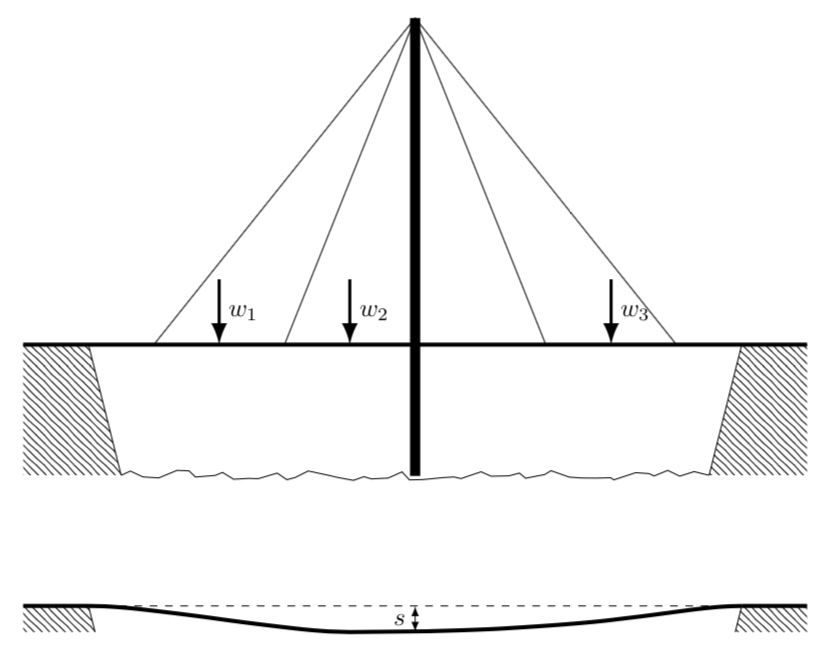
\includegraphics[width=11cm]{myndir/bru.png}}
\caption{Brú sígur þegar bílar keyra yfir hana}
\end{figure}

% Æfing

\DUadmonition[hint]{
\DUtitle[hint]{Hint}

\begin{enumerate}
\renewcommand{\labelenumi}{\alph{enumi})}
\item Tveggja tonna bíll á stöðunum þremur sem merktir eru með $w_1$,
$w_2$ og $w_3$ á myndinni að ofan veldur sigi sem er 0.24 mm,
0.31 mm og 0.26 mm. Ákvarðið stuðana $c_i, i=1,2,3$

\item Nú eru þrír bílar settir á staðina, 1.5 tonn, 0.8 tonn og 1.2
tonn. Hve mikið sígur brúin í miðjunni?
\end{enumerate}
}


\section{Taylor-nálgun%
  \label{taylor-nalgun}%
}


\subsection{Stigull af margvíðu falli%
  \label{stigull-af-margviu-falli}%
}

Með hliðsjón af setningunni um tvíðvíðan stigul í grein %
\raisebox{1em}{\hypertarget{id10}{}}\hyperlink{id9}{\textbf{\color{red}:numref:`stigull`}}
skilgreinum við stigul af $n$-víðu falli $f$ með:

\DUadmonition[system-message]{
\DUtitle[system-message]{system-message}
\raisebox{1em}{\hypertarget{id9}{}}

{\color{red}ERROR/3} in \texttt{kafli04.rst}, line~467

\hyperlink{id10}{
Unknown interpreted text role \textquotedbl{}numref\textquotedbl{}.
}}
%
\begin{equation*}
\nabla f(x) =
\begin{pmatrix}
\dfrac{\partial f(x)}{\partial x_1}\\
\vdots\\
\dfrac{\partial f(x)}{\partial x_n}
\end{pmatrix}
\end{equation*}
Hér táknar $\dfrac{\partial f(x)}{\partial x_i}$ hlutafleiðuna af $f$
með tilliti til $x_i$ ($i$-ta staks $x$). Stundum er
hlutafleiða $f$ í $x$ m.t.t. $x_i$ táknuð með $f_i(x)$.
Ef $x$ vigur settur saman úr talnabreytum t.d. $x = (u, v, w)$ eru
hlutafleiðurnar líka stundum ritaðar með því að láta breytu vera lágvísi, t.d.
$f_u$, í stað $\dfrac{\partial f}{\partial u}$. Enn einn
rithátturinn fyrir afleiðu $f$ m.t.t. $x$ er $D_x f(x,...)$.

\begin{figure}
\noindent\makebox[\linewidth][c]{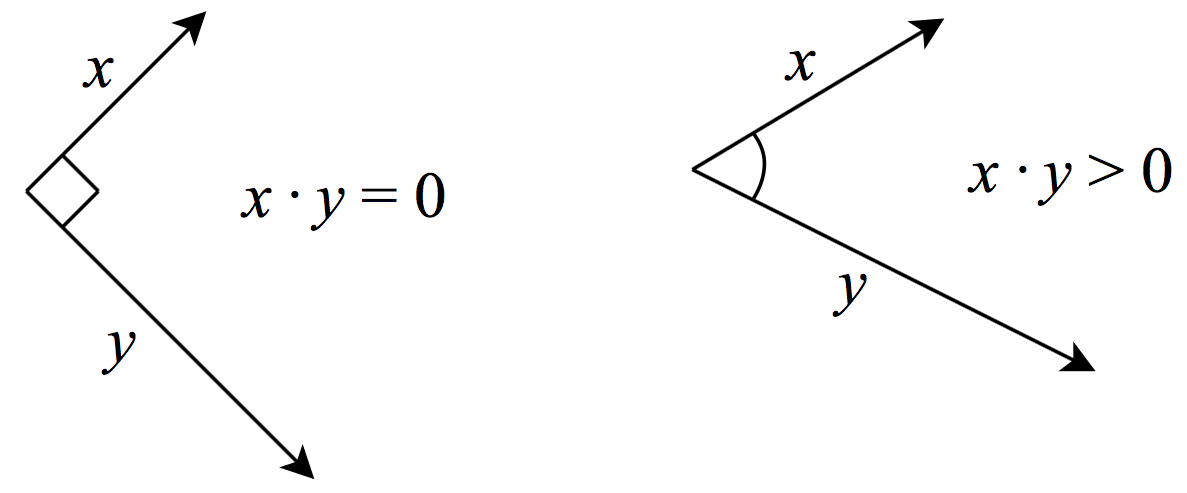
\includegraphics[width=9cm]{myndir/innfeldi.png}}
\caption{Innfeldi vigra og horn milli þeirra}
\end{figure}

% Sýnidæmi

\DUadmonition[important]{
\DUtitle[important]{Important}

Lát
%
\begin{equation*}
f(x,y,z) = xy^3 + (2x^2 - z)^2
\end{equation*}
Þá er
%
\begin{equation*}
\nabla f(x,y,z) =
\begin{pmatrix}
y^3 + 2(2x^2 - z) 4x\\
3xy^2 + 0\\
0 + 2(2x^2 - z)(-1)
\end{pmatrix} =
\begin{pmatrix}
y^3 + 8x(2x^2 - z)\\
3xy^2\\
-4x^2 + 2z
\end{pmatrix}
\end{equation*}}

% Æfing

\DUadmonition[hint]{
\DUtitle[hint]{Hint}

\begin{enumerate}
\renewcommand{\labelenumi}{\alph{enumi})}
\item Finnið $f'(x)$, $g'(x)$ og $h'(x)$ ef:
%
\begin{align*}
f(x) &= 2x^3 + 5 \\
g(x) &= 2ax^3 + b \\
h(x) &= \frac{(2x-1)^3}{3}
\end{align*}
\item Lát
%
\begin{equation*}
f(x,y,z) = xyz + x^2y^2 - (z-x)^2
\end{equation*}
Ákvarðið $\nabla f(x,y,z)$

\item Lát $f(x) = \dfrac{\sin x_1}{x_2}$. Ákvarðið $\nabla f(x)$

\item Finnið $D_z \dfrac{\exp(xyz)}{xyz}$ (munið að $D\dfrac{u}{v} =
\dfrac{u'v-v'u}{v^2}$)
\end{enumerate}
}


\subsection{Setning Taylors í einni og fleiri víddum%
  \label{setning-taylors-i-einni-og-fleiri-viddum}%
}

Ef $f$ er eitthvert gefið fall þá er ein leið til að nálga það með
línulegu falli sú að nota setningu Taylors. Einvíða útgáfuna af
henni þekkja margir nemendur, en fyrir nálgun með beinni línu hljóðar hún svona:

Ef $a$ er gefin tala og $f$ er diffranlegt fall þá gildir fyrir
$x$ nálægt $a$ að
%
\begin{equation*}
f(x) \approx f(a) + f'(a)(x-a) \;\;\; \text{(einví\eth  Taylor-setning)}
\end{equation*}
Ef $f$ er margvítt fall, $f: \Bbb{R}^n \to \Bbb{R}$, og $x$ er
vigur nálægt vigrinum $a$ þá má líka nálga $f(x)$ línulega, en nú
kemur stigull í stað afleiðu, og innfeldi í stað margföldunar:
%
\begin{equation*}
f(x) \approx f(a) + \nabla f(a) \cdot (x-a) \;\;\; \text{(margví\eth  Taylor-setning)}
\end{equation*}
Fallið $\hat{f}(x) = f(a) + \nabla f(a) \cdot (x-a)$ er nefnt
\emph{Taylor-nálgun} við $f$ í $a$.

\begin{figure}
\noindent\makebox[\linewidth][c]{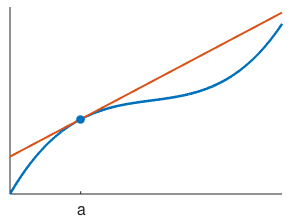
\includegraphics[width=6cm]{myndir/taylor1.png}}\phantomsection\label{taylor-lina}

\caption{Einvítt fall og línuleg Taylor-nálgun þess í $a$}
\end{figure}

Athugið að þegar $f$ er einvítt
fall þá er Taylor-nálgunin jafna beinnar línu sem snertir ferilinn sem táknar
graf fallsins í $(a,f(a))$ (sbr. %
\raisebox{1em}{\hypertarget{id12}{}}\hyperlink{id11}{\textbf{\color{red}:numref:`taylor-lína`}}), og að
þegar $f$ er tvívítt þá er hún jafna plans sem snertir yfirborðið sem
táknar graf fallsins í $(a,f(a))$.

\DUadmonition[system-message]{
\DUtitle[system-message]{system-message}
\raisebox{1em}{\hypertarget{id11}{}}

{\color{red}ERROR/3} in \texttt{kafli04.rst}, line~565

\hyperlink{id12}{
Unknown interpreted text role \textquotedbl{}numref\textquotedbl{}.
}}

% Sýnidæmi

\DUadmonition[important]{
\DUtitle[important]{Important}

Látum $f(x) = x_1 + \exp(x_2 - x_1)$ og skoðum línulega Taylor-nálgun
þess í $a = (1,2)$. Við fáum:
%
\begin{equation*}
f(a) = a_1 + \exp(a_2 - a_1) = 1 + \exp(1) = 3.718
\end{equation*}
ef reiknað er með þremur aukastöfum. Diffrun gefur svo:
%
\begin{align*}
\nabla f(x)
&=
\begin{pmatrix}
1 - \exp(x_2 - x_1)\\
\exp(x_2 - x_1)
\end{pmatrix} \\
&= (1 - \exp(1), \exp(1)) \\
&= (-1.718, 2,718)
\end{align*}
Ef þetta er sett inn í margvíðu Taylor-setninguna fæst:
%
\begin{align*}
\hat{f}(x) &= f(a) + \nabla f(a) \cdot (x - a) \\
           &= 3.718 + (-1.718, 2.718) \cdot (x_1 - 1, x_2 - 2) \\
           &= 3.718 - 1.718(x_1 - 1) + 2.718(x_2 - 2) \\
           &= -1.718x_1 + 2.718x_2
\end{align*}
Eftirfarandi tafla sýnir $f(x)$ og $\hat{f}(x)$ fyrir nokkur
gildi á $x$ í grennd við $a$

\begin{quote}
\begin{longtable*}[c]{|l|l|l|}
\hline
\textbf{$x$} & \textbf{$f(x)$} & \textbf{$\hat{f}(x)$} \\
\hline
\endfirsthead
\hline
\textbf{$x$} & \textbf{$f(x)$} & \textbf{$\hat{f}(x)$} \\
\hline
\endhead
\multicolumn{3}{c}{\hfill ... continued on next page} \\
\endfoot
\endlastfoot
$(1,2)$ & 3.7183 & 3.7183 \\
\hline
$(0.96, 1.98)$ & 3.7332 & 3.7326 \\
\hline
$(0.85, 2.05)$ & 4.17 & 4.11 \\
\hline
$(1.25, 1.41)$ & 4.44 & 4.40 \\
\hline
\end{longtable*}
\end{quote}

Við sjáum að nálgunin er bara ágæt.
}

% Æfing

\DUadmonition[hint]{
\DUtitle[hint]{Hint}

\begin{enumerate}
\renewcommand{\labelenumi}{\alph{enumi}.}
\item Ákvarðið $\hat{f}(x)$, línulega Taylor-nálgun fallsins $f(x) = 2\ln(x)+1$,
í punktinum $a=1$. Gerið töflu yfir $f(x)$ og
$\hat{f}(x)$ fyrir $x = 1, 1.1$ og $1.2$

\item Finnið línulega Taylor-nálgun við tvívíða fallið
$f(x) = x_1^2 + x_1 x_2 + x_2^2$ í punktinum $a = (1,2)$. Ákvarðið gildi
$f(x)$ og nálgunarinnar í punktinum $x = (1.1, 2.1)$.

\item Finnið Taylor-nálgun við þrívíða fallið $f(x,y,z) = xyz + x$
í punktinum $(1,1,0)$ {[}þetta er æfing í því tilviki að viðfang þrívíðs falls
sé ritað sem vigur $(x,y,z)${]}.
\end{enumerate}
}


\section{Norm og fjarlægðir%
  \label{norm-og-fjarlaegir}%
}

Í þessum kafla verður fjallað um norm, sem er mælikvarði á
stærð vigurs, og skyld hugtök, fjarlægðir og horn milli vigra.


\subsection{Skilgreining norms%
  \label{skilgreining-norms}%
}

Eins og áður hefur verið bent á er hægt að túlka tvívíða og þrívíða vigra sem
færslu í plani eða rúmi, eða ör sem hefur stefnu og lengd.

\begin{figure}
\noindent\makebox[\linewidth][c]{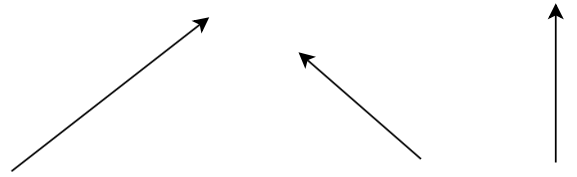
\includegraphics[width=8cm]{myndir/vigrar.png}}
\caption{Tvívíðir vigrar sýndir sem örvar (eða færslur)}
\end{figure}

Það liggur beint við að leggja mælikvarða á stærð slíkra vigra með því að mæla
lengd þeirra í rúminu. Þessa lengd má líka reikna með Pýþagórasarreglu útfrá
hnitum vigranna og þá fæst:
%
\begin{equation*}
\text{Lengd } x = \sqrt{x_1^2 + x_2^2}
\end{equation*}
Fyrir vigra í þrívíðu rúmi er hægt að beita Pýþagórasarreglu tvisvar til
að reikna lengdina og fá:
%
\begin{equation*}
\text{Lengd } x = \sqrt{x_1^2 + x_2^2 + x_3^2}
\end{equation*}
Nú liggur beint við hvernig hægt er að útvíkka þessar formúlur fyrir almenna
$n$-víða vigra. Hugtakið sem fæst er nefnt \emph{Evklíðskt norm} (\emph{Euclidean
norm}) eða 2-norm, og táknað með $\|x\|$, eða stundum $\|x\|_2$ til
að aðgreina það frá öðrum aðferðum til að skilgreina norm sem verða reyndar ekki
á dagskrá hér:

\begin{quote}
\textbf{Skilgreining} Evklíðskt norm af $n$-vigri x er
%
\begin{equation*}
\|x\| = \sqrt{x_1^2 + \ldots + x_n^2}
\end{equation*}\end{quote}

Normið er kennt við gríska stærðfræðingnn Evklíð sem skrifaði mikil verk og
sannaði margar setningar um rúmfræði.

\DUadmonition[attention]{
\DUtitle[attention]{Attention!}

Í Numpy má reikna norm vigurs \texttt{\DUrole{code}{x}} með \texttt{\DUrole{code}{np.norm(x)}}
}

\DUadmonition[attention]{
\DUtitle[attention]{Attention!}

Í \href{http://stæ.is/os}{Stærfræðiorðasafninu} er \emph{norm} þýtt með
\emph{staðall} eða \emph{lengd}, en í þessum fyrirlestrarnótum er aðeins slakað
á hreintungustefnunni.
}

% Æfing

\DUadmonition[hint]{
\DUtitle[hint]{Hint}

\begin{enumerate}
\renewcommand{\labelenumi}{\alph{enumi}.}
\item Reiknið $\|(3, 4)\|$

\item Reiknið $\|(2, -4, -5, 6)\|$

\item Sýnið að fyrir öll horn $\theta$ gildir að $\|(\sin \theta,
\cos\theta)\| = 1$
\end{enumerate}
}


\subsection{Reglur um norm%
  \label{reglur-um-norm}%
}

Hægt er að leiða út fjölmargar reglur um norm, en hér verða örfáar látnar
duga. Í eftirfarandi reglum eru $x$ og $y$ einhverjir
$n$-vigrar og $\alpha$ einhver rauntala:
%
\begin{align*}
&\|\alpha x\| = \alpha \|x\| \\
&\|x + y\| \leq \|x\| + \|y\| \text{ (þríhyrningsójafnan)} \\
&\|x\| \geq 0 \\
&\|x\| = 0 \text{ þ.þ.a.a } x = 0
\end{align*}
% Æfing

\DUadmonition[hint]{
\DUtitle[hint]{Hint}

\begin{enumerate}
\renewcommand{\labelenumi}{\alph{enumi}.}
\item Sannið fyrstu regluna.

\item Sannið þríhyrningsójöfnuna fyrir tvívíða vigra með því að teikna
viðeigandi þríhyrning, og notfæra ykkur að stysta leið
milli tveggja punkta er bein lína.
\end{enumerate}
}


\subsection{Fjarlægðir%
  \label{fjarlaegir}%
}

Ef $a$ og $b$ eru tveir punktar í plani eða þrívíðu rúmi þá er vigur
frá $a$ til $b$ gefinn með $b - a$:

\begin{figure}
\noindent\makebox[\linewidth][c]{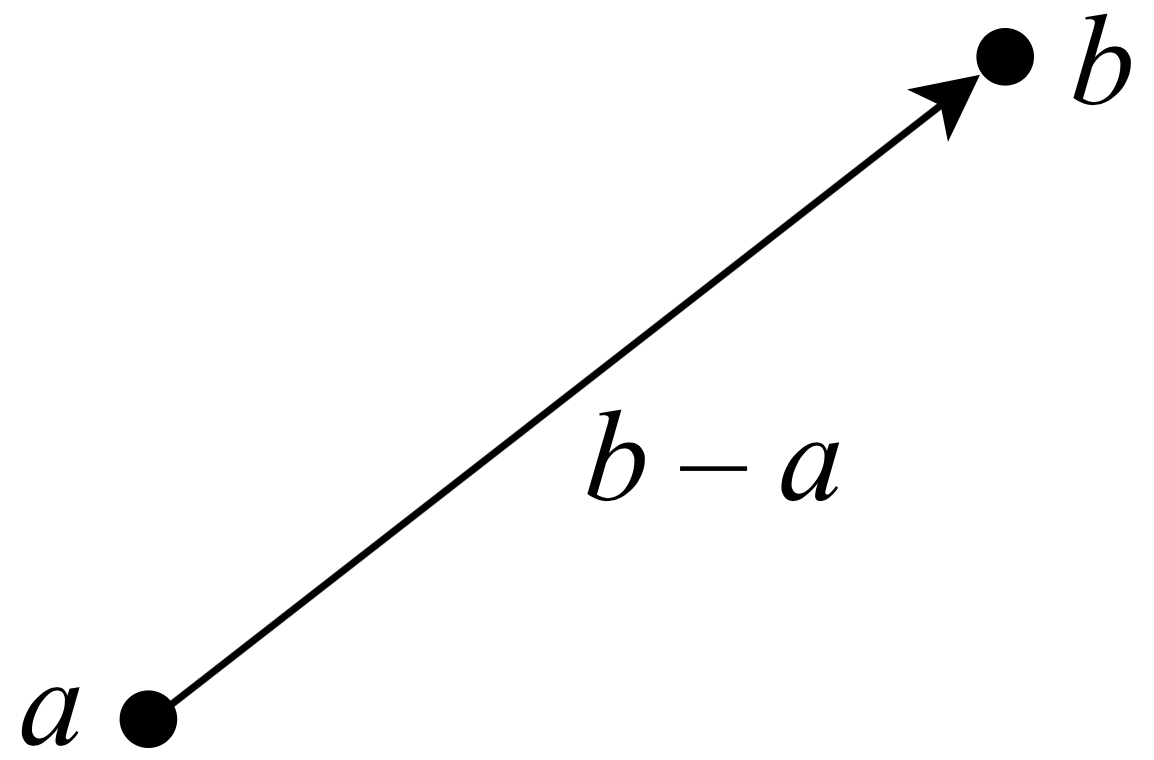
\includegraphics[width=5cm]{myndir/fjarlægð.png}}\end{figure}

og þessvegna er fjarlægðin milli $a$ og $b$ gefin með
$\|b-a\|$, eða $\|a-b\|$ sem er jafngilt. Því liggur beint við
að skilgreina fjarlægð milli almennra vigra á sama hátt.

\begin{quote}
\textbf{Skilgreining:} Ef $a$ og $b$ eru $n$-vigrar þá er
fjarlægðin milli $a$ og $b$ gefin með:
%
\begin{equation*}
\|a-b\|
\end{equation*}\end{quote}

Ekki er erfitt að sjá að ef lítill munur er á tilsvarandi stökum tveggja vigra
þá verður fjarlægðin á milli þeirra lítil tala.

% Sýnidæmi

\DUadmonition[important]{
\DUtitle[important]{Important}

Fjarlægðin á milli vigranna $x = (2,3,5,5)$ og $y = (1,1,1,-5)$ er
%
\begin{align*}
\|x-y\| &= \|(1,2,4,10)\| \\
&= \sqrt{1^2 + 2^2 + 4^2 + 10^2}
&= \sqrt{121}
&= 11
\end{align*}}

Fjarlægðir milli vigra koma við sögu í ýmsum verkefnum í reiknifræði, og ýmsum
reikniritum, t.d. hinu velþekkta \emph{k-means} reikniriti sem fjallað verður um
síðar í þessum fyrirlestrarnótum, og sömuleiðis í verkefnum í máltækni t.d. í
samanburði tveggja texta, eins og sýnt verður í næstu grein.


\subsection{Orðtíðni og fjarlægð milli vigra%
  \label{ortini-og-fjarlaeg-milli-vigra}%
  \label{ortini}%
}

Orðtíðnivigur fyrir skjal (eða vefsíðu) er gerður þannig að hvert orð
í skjalinu er fært yfir á staðalsnið (t.d. nefnifall eintölu fyrir
nafnorð), orðunum er raðað í stafrófsröð, og svo er talið hve oft hvert
orð kemur fyrir. Oft er algengum orðum (t.d. og, er, á, í) sleppt og líka
sjaldgæfum. Tökum sem dæmi vísupartinn:

\begin{quote}
Ástin er eins og sinueldur. 
Ástin er segulstál. 
Af litlum neista verður oft mikið bál. 
Ástin er eins og hvítigaldur, 
gagntekur líkama’ og sál.
\end{quote}

Orðtíðnirit fyrir hana gæti verið:

\begin{quote}
\begin{longtable*}[c]{|l|l|l|}
\hline
ást & 3 & 0.30 \\
\hline
bál & 1 & 0.10 \\
\hline
eins & 2 & 0.20 \\
\hline
líkami & 1 & 0.10 \\
\hline
lítill & 1 & 0.10 \\
\hline
mikið & 1 & 0.10 \\
\hline
neisti & 1 & 0.10 \\
\hline
\end{longtable*}
\label{ortinitafla}
\end{quote}

og miðdálkurinn gefur orðtíðnivigur. Ef bera á saman tvö eða fleiri skjöl er
búinn til sameiginlegur orðalisti fyrir þau öll áður en orðin eru talin, og ef
skjölin eru mislöng þá er sennilega betra að reikna orðtíðnina hlutfallslega,
eins og í aftasta dálkinum í töflunni að ofan. Tvö skjöl sem fjalla um sama eða
svipuð efni eru líklegri til að hafa stutt á milli orðtíðnivigra sinna heldur en
skjöl um ólík efni.

% Sýnidæmi

\DUadmonition[important]{
\DUtitle[important]{Important}

Búnir voru til orðtíðnivigrar fyrir þrjár greinar á Wikipediu, um
Óskarsverðlaunin, Golden-globe-verðlaunin, og ofurskálina, og fjarlægðirnar
á milli þeirra reiknaðar. Niðurstaðan var:

\begin{longtable*}[c]{|l|l|l|l|}
\hline
 & Óskarsverðlaun & Golden-globe & Ofurskál \\
\hline
Óskarsverðlaun & 0 & 0.11 & 0.17 \\
\hline
Golden-globe & 0.11 & 0 & 0.18 \\
\hline
Ofurskál & 0.17 & 0.18 & 0 \\
\hline
\end{longtable*}

Hér sést að fjarlægðin milli greinanna um verðlaunin er minna en fjarlægðin frá
þeim yfir í ofurskálargreinina.
}


\subsection{Horn milli vigra%
  \label{horn-milli-vigra}%
}

Í tvívíðu og þrívíðu rúmi er hægt að reikna horn milli tveggja vigra
rúmfræðilega útfrá innfeldi og normum vigranna. Formúlan sem
hægt er að sanna fyrir $n = 2$ og $n = 3$, er sú sem gefin er
í eftirfarandi skilgreininingu, sem útvíkkar sem sé hugtakið \emph{horn} þegar
$n > 3$:

\begin{quote}
\textbf{Skilgreining:} Ef $x$ og $y$ eru $n$-vigrar þá er
\emph{hornið} milli þeirra gefið með
%
\begin{equation*}
\theta = \arccos \frac{x \cdot y}{\|x\|\, \|y\|}
\end{equation*}\end{quote}

\textbf{Horn og líkindi með vigrum}. Í staðinn fyrir að mæla fjarlægð milli
orðtíðnivigra er hægt að nota hornið á milli þeirra til að meta líkindi með
tveimur skjölum eða vefsíðum.

% Sýnidæmi

\DUadmonition[important]{
\DUtitle[important]{Important}

Í eftirfarandi töflu hafa hornin milli
orðtíðnivigra Wikipedíuskjalanna sem voru rædd í grein %
\raisebox{1em}{\hypertarget{id14}{}}\hyperlink{id13}{\textbf{\color{red}:numref:`orðtíðni`}} verið
reiknuð.

\DUadmonition[system-message]{
\DUtitle[system-message]{system-message}
\raisebox{1em}{\hypertarget{id13}{}}

{\color{red}ERROR/3} in \texttt{kafli04.rst}, line~869

\hyperlink{id14}{
Unknown interpreted text role \textquotedbl{}numref\textquotedbl{}.
}}

\begin{longtable*}[c]{|l|l|l|l|}
\hline
 & Óskarsverðlaun & Golden-globe & Ofurskál \\
\hline
Óskarsverðlaun & 0 & 59° & 87° \\
\hline
Golden-globe & 59° & 0 & 86° \\
\hline
Ofurskál & 87° & 86° & 0 \\
\hline
\end{longtable*}

Við sjáum að eins og í grein %
\raisebox{1em}{\hypertarget{id16}{}}\hyperlink{id15}{\textbf{\color{red}:numref:`orðtíðni`}} eru verðlaunagreinarnar mun nær
hvor annarri en ofurskálargreininni samkvæmt hornmælikvarðanum. Öfugt við
fjarlægðarkvarðann þá er óþarfi að reikna hlutfallslega orðtíðni því sömu horn
fást með því að nota orðtíðnina beint (t.d. miðdálkinn í (fyrri) töflunni
í grein %
\raisebox{1em}{\hypertarget{id18}{}}\hyperlink{id17}{\textbf{\color{red}:numref:`orðtíðni`}}).

\DUadmonition[system-message]{
\DUtitle[system-message]{system-message}
\raisebox{1em}{\hypertarget{id15}{}}

{\color{red}ERROR/3} in \texttt{kafli04.rst}, line~896

\hyperlink{id16}{
Unknown interpreted text role \textquotedbl{}numref\textquotedbl{}.
}}

\DUadmonition[system-message]{
\DUtitle[system-message]{system-message}
\raisebox{1em}{\hypertarget{id17}{}}

{\color{red}ERROR/3} in \texttt{kafli04.rst}, line~896

\hyperlink{id18}{
Unknown interpreted text role \textquotedbl{}numref\textquotedbl{}.
}}
}

% Æfing

\DUadmonition[hint]{
\DUtitle[hint]{Hint}

\begin{enumerate}
\renewcommand{\labelenumi}{\alph{enumi}.}
\item Reiknið hornið á milli vigranna $(4,3)$ og $(1,0)$.

\item Notið regluna um kósínus af mismun,
%
\begin{equation*}
\cos(a - b) = \cos a\cos b + \sin a \sin b
\end{equation*}
til að sýna að skilgreiningin á horni milli $x$ og $y$ að framan
gefur rúmfræðilega hornið þegar vigrarnir eru tvívíðir.

\begin{quote}
\textbf{Leiðbeining:} \emph{Hornið á milli vigranna er mismunur stefnuhorna þeirra. Í pólhnitum
verða hnit} $x$ \emph{og} $y$:
%
\begin{align*}
x_1 &= r\cos a \qquad y_1 &= R \cos b\\
x_2 &= r \sin a \qquad y_2 &= R \sin b
\end{align*}
\emph{þar sem} $r = \|x\|$, $R = \|y\|$, $a = {}$
\emph{stefnuhorn} $x$ \emph{og} $b = {}$ \emph{stefnuhorn} $y$.
\end{quote}
\end{enumerate}
}


\section{Tölfræðileg föll af vigrum%
  \label{tolfraeileg-foll-af-vigrum}%
}


\subsection{Meðaltal, dreifni og staðalfrávik%
  \label{mealtal-dreifni-og-staalfravik}%
}

$\newcommand{\Var}{\operatorname{Var}}$
$\newcommand{\std}{\operatorname{std}}$ Meðaltal (\emph{mean}), dreifni
:math:(\emph{variance}) og staðalfrávik (\emph{standard deviation}). eru hugtök í tölfræði
:math:sem eru samt nátengd vigrum og línulegri algebru.

\begin{quote}
\textbf{Skilgreining:} \emph{Meðaltal} $n$-vigurs $x$ er gefið með
%
\begin{equation*}
\overline{x} = \frac{1}{n}\sum_{i=1}^n x_i
\end{equation*}
\textbf{Skilgreining:} \emph{Dreifni} $n$-vigurs $x$ er gefin með
%
\begin{equation*}
\Var{x} = \frac{1}{n}\sum_{i=1}^n (x_i - \overline{x})^2
\end{equation*}
\textbf{Skilgreining:} \emph{Staðaðfrávik} $n$-vigurs $x$ er gefið með
%
\begin{equation*}
\std{x} = \sqrt{\Var{x}} = \sqrt{\frac{1}{n}\sum_{i=1}^n (x_i -
\overline{x})^2}
\end{equation*}\end{quote}

Dreifni og staðalfrávik eru mælikvarði á það hve langt frá meðaltalinu einstök
stök vigursins eru að jafnaði. Í staðinn fyrir að leggja saman önnur veldi af
fráviki frá meðaltali væri mögulegt að leggja í saðinn saman tölugildi
frávikanna, $\frac{1}{n}\sum_{i=1}^n |x_i - \overline{x}|$, en ýmsar
ástæður, bæði tölfræðilegar og reiknitæknilegar, mæla gegn því.

\textbf{Reglur um staðalfrávik.} Ef $x$ er $n$-vigur og $a$ er rauntala þá gilda eftirfarandi
reglur um staðalfrávik:
%
\begin{align*}
&{\bf 1.}\;\,\text{Ef } y_i = x_i + a \text{ fyrir öll } i \text{ þá er } \std(y) =
\std(x)\\
&{\bf 2.}\;\std(ax) = |a|\std(x)
\end{align*}
Það breytir sem sagt ekki staðalfráviki að leggja fasta við öll stök
vigurs, og ef vigur er margfaldaður með tölu, þá margfaldast staðalfrávikið með
tölugildinu af tölunni.

\DUadmonition[attention]{
\DUtitle[attention]{Attention!}

Með Numpy má reikna meðaltal, dreifni og staðalfrávik \texttt{\DUrole{code}{x}} með
\texttt{\DUrole{code}{np.mean(x)}}, \texttt{\DUrole{code}{np.var}} og \texttt{\DUrole{code}{np.std}}.
}


\subsection{Stöðlun%
  \label{stolun}%
}

Stundum hentar að staðla (\emph{standardize}) gögn, en þá er meðaltal þeirra dregið
frá og deilt með staðalfrávikinu, og þannig fæst útgáfa af gögnunum sem hefur
meðaltal 0 og staðalfrávik 1. Stöðluð útgáfa vigurs $x$ er stundum gefið
nafnið $z$ og/eða kölluð \emph{z-stig} (\emph{z-score}), sérstaklega ef $x$ er
vigur af normaldreifðum gögnum.

\begin{quote}
\begin{quote}
\textbf{Skilgreining:} \emph{Stöðlun} (\emph{standardization}) vigurs $x$ hefur
$i$-ta stak
\end{quote}
%
\begin{equation*}
z_i = \frac{x_i - \overline{x}}{\std(x)}
\end{equation*}\end{quote}

Hægt er að hugsa sér að $z_i$ mæli hve mörgum staðalfrávikum fyrir ofan
eða neðan meðaltalið $x_i$ er. Skylt þessu er þegar búnir eru til
mælikvarðar með meðaltal og staðalfrávik sem eru rúnnaðar tölur, t.d.
greindarvísitala sem skv. skilgreiningu hefur meðaltal 100 og staðalfrávik 15.

% Æfing

\DUadmonition[hint]{
\DUtitle[hint]{Hint}

\begin{enumerate}
\renewcommand{\labelenumi}{\alph{enumi}.}
\item Ákvarðið meðaltal, dreifni og staðalfrávik vigursins
$x = (2, 3, 4, 6)$

\item Ákvarðið í framhaldi staðlaða útgáfu af $x$

\item Notið a-lið og reglur um staðalfrávik til að reikna staðalfrávik vigranna
$y = (4,5,6,8)$ og $z = -3x$
\end{enumerate}
}


\subsection{Fylgni%
  \label{fylgni}%
}

Fylgnistuðull eða fylgni (\emph{correlation (coefficient)}) er líka tölfræðilegt
hugtak tengt línulegri algebru og vigrum. Reyndar eru til nokkrar leiðir til að
reikna fylgni, en sú langalgengasta er að nota fylgnistuðul Pearsons og það er
gert hér. Um hann má lesa nánar t.d. á
\href{https://en.wikipedia.org/wiki/Pearson_correlation_coefficient//}{Wikipedíu}.
Fylgni mælir samband tveggja vigra, hann er á bilinu $[-1,1]$ og hann er
$-1$ eða $1$ ef skatterplot af vigrunum liggur á beinni línu, og
$0$ ef jafna bestu línu fyrir slíkt plot er lárétt.

\begin{quote}
\textbf{Skilgreining:} \emph{Fylgnistuðull} tveggja $n$-vigra $x$ og
$y$ er gefinn með:
%
\begin{equation*}
r_{xy} = \frac{\sum_{i=1}^n (x_i - \overline{x})(y_i -
\overline{y})}{\std(x) \std(y)}
\end{equation*}\end{quote}

\DUadmonition[attention]{
\DUtitle[attention]{Attention!}

Til að reikna fylgni í Python má nota tölfræðipakkann í Scipy, t.d.:

\begin{DUclass}{code}
\begin{DUclass}{python}
\begin{quote}
\ttfamily\raggedright
\DUrole{keyword}{\DUrole{namespace}{import}}~\DUrole{name}{\DUrole{namespace}{scipy.stats}}~\DUrole{keyword}{\DUrole{namespace}{as}}~\DUrole{name}{\DUrole{namespace}{stat}}~\\
\DUrole{name}{x}~\DUrole{operator}{=}~\DUrole{name}{np}\DUrole{operator}{.}\DUrole{name}{array}\DUrole{punctuation}{({[}}\DUrole{literal}{\DUrole{number}{\DUrole{integer}{1}}}\DUrole{punctuation}{,}~\DUrole{literal}{\DUrole{number}{\DUrole{integer}{2}}}\DUrole{punctuation}{,}~\DUrole{literal}{\DUrole{number}{\DUrole{integer}{3}}}\DUrole{punctuation}{{]})}~\\
\DUrole{name}{y}~\DUrole{operator}{=}~\DUrole{name}{np}\DUrole{operator}{.}\DUrole{name}{array}\DUrole{punctuation}{({[}}\DUrole{literal}{\DUrole{number}{\DUrole{integer}{2}}}\DUrole{punctuation}{,}~\DUrole{literal}{\DUrole{number}{\DUrole{integer}{3}}}\DUrole{punctuation}{,}~\DUrole{literal}{\DUrole{number}{\DUrole{integer}{4}}}\DUrole{punctuation}{{]})}~\\
\DUrole{name}{r}\DUrole{punctuation}{,}\DUrole{name}{p}~\DUrole{operator}{=}~\DUrole{name}{stat}\DUrole{operator}{.}\DUrole{name}{pearsonr}\DUrole{punctuation}{(}\DUrole{name}{x}\DUrole{punctuation}{,}\DUrole{name}{y}\DUrole{punctuation}{)}
\end{quote}
\end{DUclass}
\end{DUclass}

Hér skilar \texttt{\DUrole{code}{r}} fylgnistuðlinum, og \texttt{\DUrole{code}{p}} marktæknistigi hans eða
$p$-gildi, sem í grófum dráttum eru líkurnar á að fá fylgni sem er
$r$ eða meiri að tölugildi fyrir tilviljun, ef vigrarnir tveir væru
slembivigrar úr óháðum normaldreifingum.
}

\DUadmonition[hint]{
\DUtitle[hint]{Hint}

Eftirfarandi forritsbútur skilgreinir fall til að búa til tvo vigra sem hafa fylgni
u.þ.b. r. Afritið forritsbútinn yfir í Júpíter og keyrið hann.

\begin{DUclass}{code}
\begin{DUclass}{python}
\begin{quote}
\ttfamily\raggedright
\DUrole{keyword}{\DUrole{namespace}{import}}~\DUrole{name}{\DUrole{namespace}{numpy}}~\DUrole{keyword}{\DUrole{namespace}{as}}~\DUrole{name}{\DUrole{namespace}{np}}\DUrole{operator}{,}~\DUrole{name}{\DUrole{namespace}{scipy.stats}}~\DUrole{keyword}{\DUrole{namespace}{as}}~\DUrole{name}{\DUrole{namespace}{stat}}~\\
\DUrole{keyword}{\DUrole{namespace}{import}}~\DUrole{name}{\DUrole{namespace}{matplotlib.pyplot}}~\DUrole{keyword}{\DUrole{namespace}{as}}~\DUrole{name}{\DUrole{namespace}{plt}}\DUrole{operator}{,}~\DUrole{name}{\DUrole{namespace}{numpy.random}}~\DUrole{keyword}{\DUrole{namespace}{as}}~\DUrole{name}{\DUrole{namespace}{rnd}}~\\
\DUrole{name}{np}\DUrole{operator}{.}\DUrole{name}{set\_printoptions}\DUrole{punctuation}{(}\DUrole{name}{precision}\DUrole{operator}{=}\DUrole{literal}{\DUrole{number}{\DUrole{integer}{2}}}\DUrole{punctuation}{,}~\DUrole{name}{floatmode}\DUrole{operator}{=}\DUrole{literal}{\DUrole{string}{\DUrole{single}{'fixed'}}}\DUrole{punctuation}{,}~\DUrole{name}{suppress}\DUrole{operator}{=}\DUrole{name}{\DUrole{builtin}{\DUrole{pseudo}{True}}}\DUrole{punctuation}{)}~\\
~\\
\DUrole{keyword}{def}~\DUrole{name}{\DUrole{function}{tvinormal}}\DUrole{punctuation}{(}\DUrole{name}{r}\DUrole{punctuation}{,}\DUrole{name}{n}\DUrole{punctuation}{):}~\\
~~~~\DUrole{literal}{\DUrole{string}{\DUrole{doc}{\textquotedbl{}\textquotedbl{}\textquotedbl{}skilar~tveimur~n-vigrum~með~meðaltal~0,~dreifni~1,\\
~~~~~~~og~fylgni~r~(um~það~bil)\textquotedbl{}\textquotedbl{}\textquotedbl{}}}}~\\
~~~~\DUrole{name}{mu}~\DUrole{operator}{=}~\DUrole{name}{np}\DUrole{operator}{.}\DUrole{name}{array}\DUrole{punctuation}{({[}}\DUrole{literal}{\DUrole{number}{\DUrole{integer}{0}}}\DUrole{punctuation}{,}\DUrole{literal}{\DUrole{number}{\DUrole{integer}{0}}}\DUrole{punctuation}{{]})}~\\
~~~~\DUrole{name}{Sig}~\DUrole{operator}{=}~\DUrole{name}{np}\DUrole{operator}{.}\DUrole{name}{array}\DUrole{punctuation}{({[}{[}}\DUrole{literal}{\DUrole{number}{\DUrole{integer}{1}}}\DUrole{punctuation}{,}\DUrole{name}{r}\DUrole{punctuation}{{]},{[}}\DUrole{name}{r}\DUrole{punctuation}{,}\DUrole{literal}{\DUrole{number}{\DUrole{integer}{1}}}\DUrole{punctuation}{{]}{]})}~\\
~~~~\DUrole{punctuation}{(}\DUrole{name}{x}\DUrole{punctuation}{,}\DUrole{name}{y}\DUrole{punctuation}{)}~\DUrole{operator}{=}~\DUrole{name}{rnd}\DUrole{operator}{.}\DUrole{name}{multivariate\_normal}\DUrole{punctuation}{(}\DUrole{name}{mu}\DUrole{punctuation}{,}\DUrole{name}{Sig}\DUrole{punctuation}{,}\DUrole{name}{n}\DUrole{punctuation}{)}\DUrole{operator}{.}\DUrole{name}{T}~\\
~~~~\DUrole{keyword}{return}~\DUrole{name}{x}\DUrole{punctuation}{,}\DUrole{name}{y}
\end{quote}
\end{DUclass}
\end{DUclass}

\begin{enumerate}
\renewcommand{\labelenumi}{\alph{enumi}.}
\item Bætið við skipunum sem búa til tvo tíu staka vigra með fylgni u.þ.b. 0.9
og reikna og prenta út raunverulega fylgni þeirra. Prentið líka út vigrana
hlið við hlið (notið \texttt{\DUrole{code}{np.\_c{[}{]}}} sbr. grein
%
\raisebox{1em}{\hypertarget{id20}{}}\hyperlink{id19}{\textbf{\color{red}:numref:`teikning-punktasafns`}}). Keyrið nokkrum sinnum. Prófið líka
100-staka vigra. Takið eftir að ef \texttt{\DUrole{code}{x{[}i{]}}} er stórt þá er
\texttt{\DUrole{code}{y{[}i{]}}} oftast stórt líka og öfugt.

\DUadmonition[system-message]{
\DUtitle[system-message]{system-message}
\raisebox{1em}{\hypertarget{id19}{}}

{\color{red}ERROR/3} in \texttt{kafli04.rst}, line~1055

\hyperlink{id20}{
Unknown interpreted text role \textquotedbl{}numref\textquotedbl{}.
}}

\item Búið líka til reit til að búa til 500-staka vigra með fylgni u.þ.b. 0.9 og
teiknið þá með \texttt{\DUrole{code}{plt.scatter}} (sbr. grein %
\raisebox{1em}{\hypertarget{id22}{}}\hyperlink{id21}{\textbf{\color{red}:numref:`einfaldar-myndir`}} og
töflu %
\raisebox{1em}{\hypertarget{id24}{}}\hyperlink{id23}{\textbf{\color{red}:numref:`scatterstýring`}}; hæfilegt er að nota punktastærð 3).
Endurtakið fyrir nokkur mismunandi gildi á r (t.d. -0.99, 0, 0.4, 0.99).

\DUadmonition[system-message]{
\DUtitle[system-message]{system-message}
\raisebox{1em}{\hypertarget{id21}{}}

{\color{red}ERROR/3} in \texttt{kafli04.rst}, line~1062

\hyperlink{id22}{
Unknown interpreted text role \textquotedbl{}numref\textquotedbl{}.
}}

\DUadmonition[system-message]{
\DUtitle[system-message]{system-message}
\raisebox{1em}{\hypertarget{id23}{}}

{\color{red}ERROR/3} in \texttt{kafli04.rst}, line~1062

\hyperlink{id24}{
Unknown interpreted text role \textquotedbl{}numref\textquotedbl{}.
}}
\end{enumerate}
}


\section{Grunnar og línulega háðir og óháðir vigrar%
  \label{grunnar-og-linulega-hair-og-ohair-vigrar}%
}


\subsection{Línulega háðir vigrar%
  \label{linulega-hair-vigrar}%
}

\begin{quote}
\textbf{Skilgreining:} Ef $x_1$,..., $x_k$ eru vigrar og
$c_1$,..., $c_k$ eru tölur þá er vigurinn
%
\begin{equation*}
y = c_1 x_1 + \ldots + c_k x_k
\end{equation*}
kallaður \emph{línuleg samantekt} (\emph{linear combination}) af vigrunum
$x_1$,..., $x_k$
\end{quote}

Mengi allra línulegra samantekta af vigrum $x_1$,..., $x_k$
er sagt vera \emph{spannað} (\emph{spanned}) af vigrunum.

% Sýnidæmi

\DUadmonition[important]{
\DUtitle[important]{Important}

Ef $u = (1,1,0)$ og $v = (0,0,1)$ þá er $y = 3u + 2v$
línuleg samantekt af $u$ og $v$. Mengið sem $u$ og
$v$ spanna er lóðrétta planið í gegn um línuna $y = x$.
Þetta mengi má rita:
%
\begin{equation*}
\{w \in \Bbb{R}^3 |\; w = au + bv \text{ fyrir einhver } a,b \in \Bbb{R}\}
\end{equation*}
Hér er mynd sem sýnir þessa vigra og tilheyrandi spannplan:

\begin{figure}
\noindent\makebox[\linewidth][c]{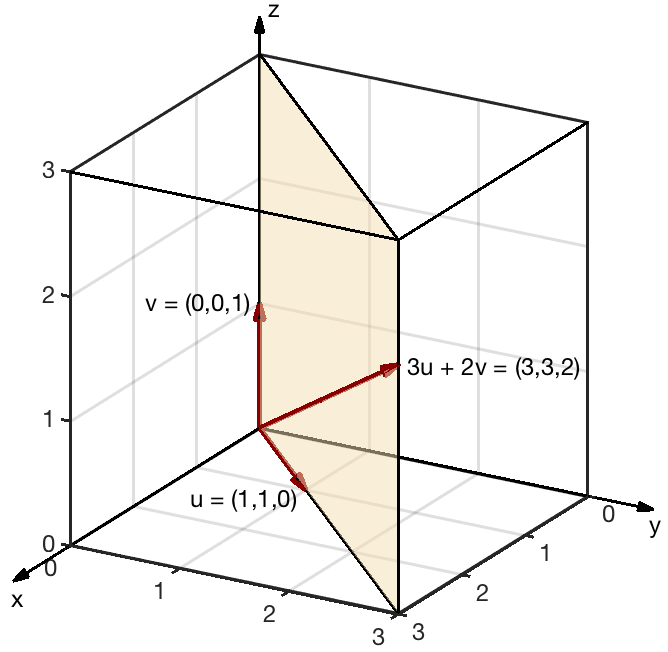
\includegraphics[width=11cm]{myndir/plotspan.png}}\end{figure}
}

Skilgreinum nú línulega háða (\emph{linearly dependent}) vigra.

\begin{quote}
\textbf{Skilgreining:} Vigrar $x_1$,..., $x_k$ eru sagðir \emph{línulega
háðir} ef hægt er að rita einhvern þeirra sem línulega samantekt af hinum,
þ.e.a.s. ef til eru tölur $c_i$ þannig að:
%
\begin{align*}
x_j = \sum_{i=1\\i \neq j}^k c_i x_i
\end{align*}\end{quote}

Rauðu vigrarnir þrír á myndinni í sýnidæminu hér á undan eru sem sé línulega
háðir, því $3u + 2v$ er línuleg samantekt af $u$ og $v$. Það
er ekki mjög erfitt að sjá að þrír vigrar í þrívíðu rúmi sem allir liggja í sama
plani hljóta að vera línulega háðir. Um tvo samsíða vigra (sem liggja þar með á
sömu línu), hvort sem er í tvívíðu eða þrívíðu rúmi, gildir að þeir eru línulega
háðir.

Ef $A$ er mengi af vigrum er talað um að það sé línulega háð ef vigrarnir
í því eru línulega háðir. Stundum er skilyrðið í skilgreiningunni orðað
öðruvísi, sbr. eftirfarandi setningu.

\begin{quote}
\textbf{Setning:} $x_1$,..., $x_k$ eru línulega háðir þ.þ.a.a. til
séu tölur $c_1,\ldots, c_k$ sem eru ekki allar $0$ þannig að
$c_1 x_1 + \ldots + c_k x_k = 0$
\end{quote}

Vigrar eru sem sé línulega háðir þ.þ.a.a. til sé línuleg samantekt af þeim sem
er núllvigurinn, með samantektarstuðlum sem eru ekki allir 0.


\subsection{Línulega óháðir vigrar%
  \label{linulega-ohair-vigrar}%
}

\begin{quote}
\textbf{Skilgreining:} Vigrar $x_1$,..., $x_k$ eru sagðir \emph{línulega
óháðir} (\emph{lindearly independent}) ef þeir eru ekki línulega háðir.
\end{quote}

Skv. setningunni að framan gildir sem sé að ef eina leiðin til að búa til
línulega samantekt af vigrum sem er núll er sú að velja alla samantektarstuðlana
sama sem núll þá eru vigrarnir línulega óháðir, en annars ekki.
Þetta gefur okkur aðferð til að sanna að mengi vigra sé línulega óháð:
Við byrjum á að rita:

\begin{quote}%
\begin{equation*}
c_1 x_1 + \ldots + c_k x_k = 0
\end{equation*}\end{quote}

og sýnum að það leiði til $c_1 = c_2 = \ldots = a_k = 0$

% Sýnidæmi

\DUadmonition[important]{
\DUtitle[important]{Important}

Sýnum að $u=(1,2,3)$, $v=(1,0,3)$ og $w=(0,1,1)$ séu
línulega óháðir. G.r.f. að \texttt{\DUrole{code}{c\_1u + c\_2v + c\_3w = 0}} sem sé
%
\begin{equation*}
c_1\begin{pmatrix}1\\2\\3\end{pmatrix} +
c_2\begin{pmatrix}1\\0\\3\end{pmatrix} +
c_3\begin{pmatrix}0\\1\\1\end{pmatrix} =
\begin{pmatrix}0\\0\\0\end{pmatrix}
\end{equation*}
Þetta gefur
%
\begin{align*}
&(1)\quad c_1 + c_2 = 0,\\
&(2)\quad 2c_1 + c_3 = 0 \text{ og}\\
&(3)\quad 3c_1 + 3c_2 + c_3 = 0.
\end{align*}
Af $(3) - 3\cdot(1)$ fæst $c_3=0$, svo $(2)$ gefur
$c_1=0$ sem með $(1)$ gefur að lokum $c_2=0$. Þetta sýnir
að $u$, $v$ og $w$ eru línulega óháðir.
}

Tveir vigrar eru sagðir samsíða ef annar er margfeldi af hinum, og eins og að
framan segir er par af ekki-núll vigrum línulega háð ef þeir eru samsíða, en
annars er parið línulega óháð (þetta er bein afleiðing af skilgreiningu á
línulega háðum vigrum).

% Æfing

\DUadmonition[hint]{
\DUtitle[hint]{Hint}

\begin{enumerate}
\renewcommand{\labelenumi}{\alph{enumi}.}
\item Skrifið vigurinn $(8,3)$ sem línulega samantekt af $(4,1)$ og
$(0,1)$.

\item Eru eftirfarandi pör vigra línulega óháð?
.. math:

\DUadmonition[system-message]{
\DUtitle[system-message]{system-message}


{\color{red}ERROR/3} in \texttt{kafli04.rst}, line~1178

Unexpected indentation.
backrefs: }

\begin{quote}
\begin{alltt}
&(1,2,3) \textbackslash{}text\{ og \} (2,4,6) \textbackslash{}\textbackslash{}
&(0,2,1) \textbackslash{}text\{ og \} (1,4,2) \textbackslash{}\textbackslash{}
&(0,-1,0) \textbackslash{}text\{ og \} (0,4,0) \textbackslash{}\textbackslash{}
&(1,2,3) \textbackslash{}text\{ og \} (2,3,4) \textbackslash{}\textbackslash{}
&(1,1,1) \textbackslash{}text\{ og \} (7,7,7)
\end{alltt}
\end{quote}
\end{enumerate}
}

Hér er að lokum setning sem segir að ekki sé hægt að skrifa gefinn vigur sem
línulegar samantektir óháðra vigra á fleiri en einn veg.

\begin{quote}
\textbf{Setning:} Ef $x_1$,..., $x_k$ eru línulega óháðir og
.. math:

\DUadmonition[system-message]{
\DUtitle[system-message]{system-message}


{\color{red}ERROR/3} in \texttt{kafli04.rst}, line~1189

Unexpected indentation.
backrefs: }

\begin{quote}
\begin{alltt}
y &= c_1 x_1 + \textbackslash{}ldots + c_k x_k \textbackslash{}\textbackslash{}
  &= d_1 x_1 + \textbackslash{}ldots + d_k x_k \textbackslash{}\textbackslash{}
\end{alltt}
\end{quote}

þá er $c_i = d_i$ fyrir öll $i$.
\end{quote}

\end{document}
